\begin{figure}[h!]
	\centering
	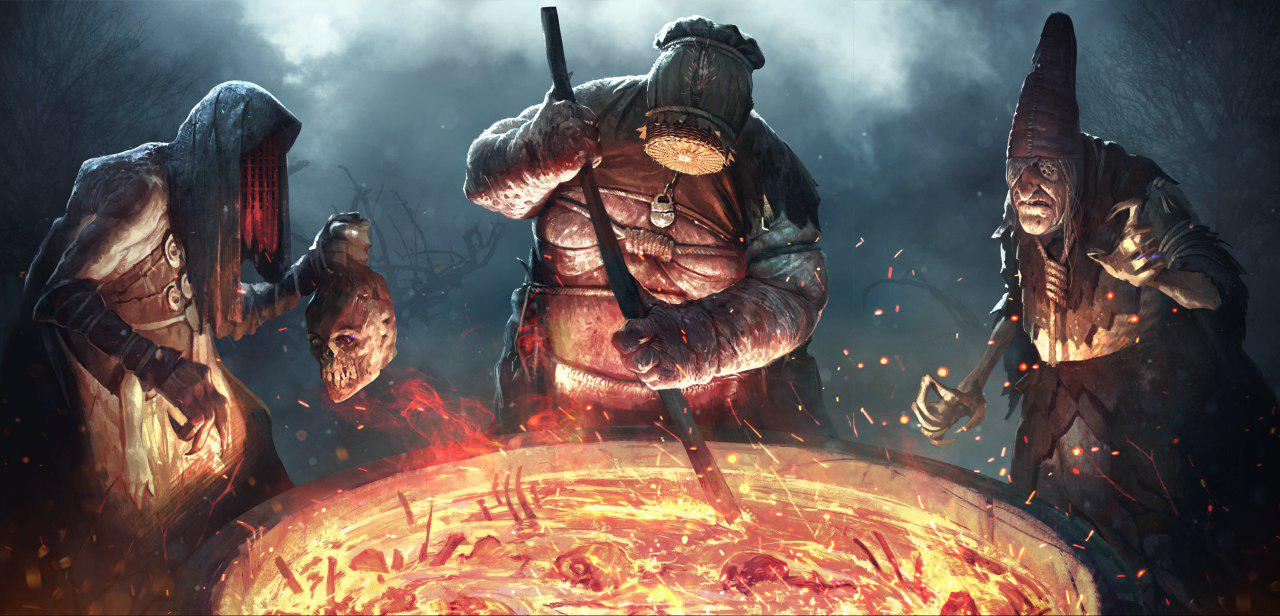
\includegraphics[width=\linewidth, keepaspectratio]{soup.jpg}
\end{figure}

Три ведьмы~---~Пряха, Кухарка и Шептуха каждое полнолуние варят себе омолаживающий супчик. 
В своей пещере на Кривоуховом болоте у самой дальней стены стоит огромный стеллаж, в каждом ящичке которого лежат неповторимые ингредиенты. 
Для того, чтобы не запутаться Шептуха присвоила каждому ящику свой индивидуальный номер~---~так, например, 
костям младенцев соответствует номер 3, любящему сердцу номер 13, а самому редкому компоненту (крови единорога)~---~666. 
Именно в день полной луны она решила пойти в деревню за новой порцией свежих детей, поэтому она оставила своим сестрам записку, где указала номера нужных ингредиентов. 
Сестры уже плохо видят в связи с довольно почтенным возрастом и из-за этого могли пару раз ошибиться. 
По возвращению Шептуха решила проверить состав их варева. Помогите ей сделать это.

\InputFile
\noindent
На вход подаются натуральные числа $N, M, K (0 < N, M \leq 100; 1 \le K \leq 30)$~---~размер котла и количество ингредиентов в нем.
На новой строке идет список нужных ингредиентов $A_1 \ldots A_K$.
Затем на вход подается двумерный массив, описывающий ингредиенты, плавающие в супчике, состоящий из натуральных чисел~---~номеров ингридиентов.


\OutputFile
\noindent

Вывести \texttt{YES}, если все элементы супа собраны правильно (т.е все нужные ингредиенты находятся в супе), и \texttt{NO}~---~если нет.

\SAMPLES